\documentclass[12pt]{article}
\usepackage{fullpage,graphicx,psfrag,amsmath,amsfonts,verbatim}
\usepackage[small,bf]{caption}
\usepackage{amsthm}
% \usepackage[hidelinks]{hyperref}
\usepackage{hyperref}
\usepackage{bbm} % for the indicator function to look good
\usepackage{color}
\usepackage{mathtools}
\usepackage{fancyhdr} % for the header
\usepackage{booktabs} % for regression table display (toprule, midrule, bottomrule)
\usepackage{adjustbox} % for regression table display
\usepackage{threeparttable} % to use table notes
\usepackage{natbib} % for bibliography
\input newcommand.tex
\bibliographystyle{apalike}
% \setlength{\parindent}{0pt} % remove the automatic indentation

\title{Empirical IO PS1}
\author{Zixuan, Anoosheh, Shuo}
\date{\today}

\begin{document}
\maketitle
\thispagestyle{empty}

% \newpage
% \thispagestyle{empty}
% \tableofcontents
% \newpage

% \setcounter{page}{1}
\section{Data}
The dataset is a panel of aggregate (model level) car sales along with the
characteristics of each model. The data spans 1977-1981 in the U.S., give rise
to 5 markets in total. We divide the quantity sold \verb|q| by the market size
(the number of households \verb|hh| in that year) to get the market share for
each model. We also adjust the car price \verb|p| by the consumer price index
\verb|cpi| to get the real price.
\begin{equation*}
    p_{adj} = \frac{100 p}{cpi}
\end{equation*}
We rescale the price by $p/1000$ to make the coefficient on price more readable.
An overview of the mean and standard deviation of the variables is shown in Table \ref{tab:desc}.
% latex table generated in R 4.3.1 by xtable 1.8-4 package
% Sat Nov  2 19:13:46 2024
\begin{table}[ht]
\centering
\begin{tabular}{rrr}
  \hline
 & mean & sd \\ 
  \hline
dpm & 0.06 & 0.02 \\ 
  door3 & 0.08 & 0.27 \\ 
  door4 & 0.52 & 0.50 \\ 
  door5 & 0.05 & 0.22 \\ 
  at & 0.28 & 0.45 \\ 
  ps & 0.38 & 0.49 \\ 
  air & 0.14 & 0.35 \\ 
  drv & 0.21 & 0.40 \\ 
  wt & 2887.27 & 702.02 \\ 
  hp2wt & 0.36 & 0.08 \\ 
  hp & 104.19 & 34.42 \\ 
  euro & 0.27 & 0.44 \\ 
  japan & 0.14 & 0.34 \\ 
  size & 1.32 & 0.24 \\ 
  wb & 104.47 & 9.14 \\ 
  p & 10.89 & 7.82 \\ 
   \hline
\end{tabular}
\end{table}


\section{Question 1:Logit}
\subsection{Utility function}
The standard utility function takes the following linear in characteristics
form:
\begin{equation}
    u_{ij}=X_{j}\beta + \alpha p_{j} + \xi_{j}+ \epsilon_{ij}=\delta_j+\epsilon_{ij}
\end{equation}
where $i$ represents individual $j$ product. And $X_{j}$ includes the following variables:\\
\verb|dpm, door3, door4, door5, at, ps, air, drv, wt, hp2wt, hp, euro, japna, size, wb, (brand dummies)|.
We assume that $\epsilon_{ij}$ is distributed type I extreme value, and are independent across all product $j$. Thus, the market share for each product is given by
By normalizing the utility of the outside good to zero, we have
\begin{equation*}
    s_j=\frac{e^{u_{ij}}}{1+\sum_{k=1}^{J}e^{u_{ik}}}
\end{equation*}
Thus,
\begin{equation}\label{eq:logit}
    \log s_j-\log s_0=\beta_0+\beta_1x_{j1}+\cdots+p_j\alpha+\xi_j
\end{equation}
where $\xi_j$ the fixed effect/unobserved heterogeneity of each product $j$.
For the remaining section, we assume that all characteristics except price are exogenous.
\subsection{Estimation}
The OLS estimation is unbiased and consistent if we assume that $\xi_j$ is
uncorrelated with $p$. We perform two ols estimation based on equation
\ref{eq:logit} with and without brand fixed effect. The results are shown in
Table \ref{tab:reg_logit}. However, it is generally not the case. Price is
generally correlated with unobserved characteristics. We construct instruments
based on \citep{blp1995}. That is, for each product characteristics $x^k$, we
compute
\begin{itemize}
    \item $z^k_{j}=\sum_{k\in \mathcal{F}_j, j'\neq j}x^k_{j'}$, the sum of characteristics of all other products belong to the same firm.
    \item $z^k_{j}=\sum_{k\notin \mathcal{F}_j}x^k_{j'}$, the sum of characteristics of all other products belong to the rival firms.
\end{itemize}
Since we have many $x^k$, we have a large number of instruments. Following \citep{blp1995}, we selected the following to instrument price $p$:\\
\verb|const_*, dpm_*, hp2wt_*,size_*, air_*|
The iv estimation results are shown in Table \ref{tab:reg_logit}.
\subsection{Results}
\begin{table}[h!]\fontsize{10pt}{12pt}\selectfont
    \centering
    
\begin{table}[htbp]
   \caption{Logit}
   \centering
   \begin{tabular}{lcccc}
      \tabularnewline \midrule \midrule
      Dependent Variable: & \multicolumn{4}{c}{log(mktshr)-log(shr\_0)}\\
      Estimator & \multicolumn{2}{c}{OLS} & \multicolumn{2}{c}{IV} \\ 
      Model:                       & (1)             & (2)             & (3)                    & (4)\\  
      \midrule
      \emph{Variables}\\
      Constant                     & -5.238$^{***}$  &                 & -5.437$^{***}$         &   \\   
                                   & (1.956)         &                 & (2.023)                &   \\   
      dpm                          & -22.04$^{***}$  & -19.04$^{***}$  & -22.57$^{***}$         & -12.95$^{**}$\\   
                                   & (4.601)         & (3.929)         & (5.125)                & (6.112)\\   
      door3TRUE                    & -0.6235$^{***}$ & -0.5271$^{***}$ & -0.6247$^{***}$        & -0.5444$^{***}$\\   
                                   & (0.2038)        & (0.1876)        & (0.2047)               & (0.1987)\\   
      door4TRUE                    & -0.0636         & -0.0190         & -0.0702                & 0.0479\\   
                                   & (0.1493)        & (0.1344)        & (0.1556)               & (0.1462)\\   
      door5TRUE                    & 0.3424          & 0.4548$^{**}$   & 0.3239                 & 0.5150$^{**}$\\   
                                   & (0.3062)        & (0.2010)        & (0.3163)               & (0.2072)\\   
      at                           & -0.2868         & -0.2917         & -0.3349                & -0.2696\\   
                                   & (0.2102)        & (0.1902)        & (0.2573)               & (0.2107)\\   
      ps                           & 0.2057          & 0.2052          & 0.2072                 & 0.1789\\   
                                   & (0.1738)        & (0.1684)        & (0.1779)               & (0.1946)\\   
      air                          & 0.1226          & -0.1486         & 0.0221                 & 0.5243\\   
                                   & (0.1797)        & (0.1689)        & (0.3451)               & (0.4311)\\   
      drv                          & 0.1029          & 0.1621          & 0.1175                 & 0.2984$^{*}$\\   
                                   & (0.1467)        & (0.1363)        & (0.1491)               & (0.1533)\\   
      wt                           & -0.0022$^{***}$ & -0.0011$^{**}$  & -0.0022$^{***}$        & -0.0012$^{*}$\\   
                                   & (0.0005)        & (0.0004)        & (0.0005)               & (0.0006)\\   
      hp2wt                        & -9.821$^{***}$  & -5.934$^{**}$   & -9.975$^{***}$         & -8.677$^{**}$\\   
                                   & (3.242)         & (2.356)         & (3.046)                & (3.761)\\   
      hp                           & 0.0381$^{***}$  & 0.0228$^{**}$   & 0.0371$^{***}$         & 0.0410$^{**}$\\   
                                   & (0.0112)        & (0.0088)        & (0.0111)               & (0.0163)\\   
      euro                         & -1.772$^{***}$  &                 & -1.938$^{***}$         &   \\   
                                   & (0.2136)        &                 & (0.5001)               &   \\   
      japan                        & -0.1290         &                 & -0.1618                &   \\   
                                   & (0.2246)        &                 & (0.2413)               &   \\   
      size                         & 2.710$^{***}$   & 0.6433          & 2.750$^{***}$          & 0.7661\\   
                                   & (0.9020)        & (0.9060)        & (0.8873)               & (1.191)\\   
      wb                           & 0.0224          & 0.0431$^{*}$    & 0.0265                 & 0.0171\\   
                                   & (0.0234)        & (0.0254)        & (0.0263)               & (0.0342)\\   
      p                            & -0.0396$^{***}$ & -0.0644$^{***}$ & -0.0213                & -0.1950$^{**}$\\   
                                   & (0.0126)        & (0.0179)        & (0.0526)               & (0.0758)\\   
      \midrule
      \emph{Fixed-effects}\\
      firmids                      &                 & Yes             &                        & Yes\\  
      \midrule
      \emph{Fit statistics}\\
      Observations                 & 501             & 501             & 501                    & 501\\  
      Adjusted R$^2$               & 0.63354         & 0.72408         & 0.63070                & 0.67282\\  
      Wald (1st stage), p          &                 &                 & 4.6332                 & 7.1002\\  
      Wald (1st stage), p-value, p &                 &                 & 0.00112                & $1.48\times 10^{-5}$\\   
      Sargan                       &                 &                 & 56.889                 & 2.6361\\  
      Sargan, p-value              &                 &                 & $2.71\times 10^{-12}$  & 0.45119\\  
      \midrule \midrule
      \multicolumn{5}{l}{\emph{Clustered (modelid) standard-errors in parentheses}}\\
      \multicolumn{5}{l}{\emph{Signif. Codes: ***: 0.01, **: 0.05, *: 0.1}}\\
   \end{tabular}
\end{table}



    \caption{Logit estimation results}
    \label{tab:reg_logit}
\end{table}

\section{Question 2:Nested logit}
\subsection{Utility function}
We relax the assumption that $\varepsilon_{ij}$ are independent across $j$.
Instead, we group the products into nests based on their size. The 3 nests are
\verb|compact, midsize, large| plus one outside option. Now the utility
function is given by
\begin{equation}
    \begin{split}
        u_{ij}&=X_{j}\beta + \alpha p_{j} + \xi_{j}+ \eta_{ig}+ \epsilon_{ij}\\
        &=\delta_j+\eta_{ig}+(1-\sigma)\epsilon_{ij}
    \end{split}
\end{equation}
Now the estimation equation is
\begin{equation}
    \log(s_j)-\log(s_0)=x_j\beta+p_j\alpha+\sigma\log(\bar{s}_{j|g})+\xi_j
\end{equation}
\subsection{Estimation}
In addition to $p$ now $\log(\bar{s}_{j|g})$ is also endogenous. We follow
\citep{berry1994} to construct additional instruments for
$\log(\bar{s}_{j|g})$, which is the sum of product characteristics of the rival
firms in the same nest $g$. The estimation results are shown in Table
\ref{tab:reg_nested_logit}.

\subsection{Results}
\begin{table}[h!]\fontsize{10pt}{12pt}\selectfont
    \centering
    
\begin{table}[htbp]
   \caption{Logit}
   \centering
   \begin{tabular}{lcccc}
      \tabularnewline \midrule \midrule
      Dependent Variable: & \multicolumn{4}{c}{log(mktshr)-log(shr\_0)}\\
      Estimator & \multicolumn{2}{c}{OLS} & \multicolumn{2}{c}{IV} \\ 
      Model:                                     & (1)             & (2)                    & (3)                    & (4)\\  
      \midrule
      \emph{Variables}\\
      Constant                                   & -4.712$^{***}$  &                        & -4.612$^{***}$         &   \\   
                                                 & (0.8660)        &                        & (1.232)                &   \\   
      dpm                                        & -8.137$^{***}$  & -9.190$^{***}$         & -12.36$^{***}$         & -17.52$^{**}$\\   
                                                 & (1.616)         & (1.561)                & (2.926)                & (6.855)\\   
      door3TRUE                                  & -0.0134         & 0.0662                 & -0.2306$^{**}$         & -0.7178$^{**}$\\   
                                                 & (0.0658)        & (0.0602)               & (0.1142)               & (0.3026)\\   
      door4TRUE                                  & -0.0311         & 0.0031                 & -0.0332                & 0.0236\\   
                                                 & (0.0569)        & (0.0511)               & (0.0791)               & (0.1726)\\   
      door5TRUE                                  & 0.1019          & 0.1758$^{**}$          & 0.2151                 & 0.5828$^{**}$\\   
                                                 & (0.0988)        & (0.0717)               & (0.1609)               & (0.2868)\\   
      at                                         & 0.0367          & -0.0741                & -0.0094                & -0.3407\\   
                                                 & (0.0969)        & (0.1086)               & (0.1263)               & (0.2534)\\   
      ps                                         & -0.1059         & -0.0123                & 0.0038                 & 0.2511\\   
                                                 & (0.0983)        & (0.1127)               & (0.1090)               & (0.2241)\\   
      air                                        & 0.0162          & -0.0004                & 0.2007                 & 0.3021\\   
                                                 & (0.0748)        & (0.0836)               & (0.1452)               & (0.3997)\\   
      drv                                        & 0.1261$^{**}$   & 0.0432                 & 0.0964                 & 0.2981\\   
                                                 & (0.0498)        & (0.0515)               & (0.0814)               & (0.1983)\\   
      wt                                         & -0.0003         & $-5.32\times 10^{-5}$  & -0.0009$^{**}$         & -0.0015$^{*}$\\   
                                                 & (0.0003)        & (0.0002)               & (0.0004)               & (0.0008)\\   
      hp2wt                                      & -1.955          & -1.307                 & -4.554$^{*}$           & -9.340$^{**}$\\   
                                                 & (1.468)         & (1.202)                & (2.487)                & (4.550)\\   
      hp                                         & 0.0104$^{**}$   & 0.0066                 & 0.0219$^{***}$         & 0.0411$^{**}$\\   
                                                 & (0.0052)        & (0.0046)               & (0.0083)               & (0.0187)\\   
      euro                                       & -0.1817$^{*}$   &                        & -0.5101$^{*}$          &   \\   
                                                 & (0.0977)        &                        & (0.2800)               &   \\   
      japan                                      & 0.0878          &                        & 0.0579                 &   \\   
                                                 & (0.0836)        &                        & (0.1300)               &   \\   
      size                                       & 1.691$^{***}$   & 1.059$^{**}$           & 1.998$^{***}$          & 0.6089\\   
                                                 & (0.4538)        & (0.4710)               & (0.5905)               & (1.259)\\   
      wb                                         & 0.0003          & 0.0107                 & 0.0022                 & 0.0336\\   
                                                 & (0.0111)        & (0.0112)               & (0.0151)               & (0.0371)\\   
      p                                          & -0.0165$^{***}$ & -0.0142                & -0.0516$^{**}$         & -0.1755$^{**}$\\   
                                                 & (0.0058)        & (0.0095)               & (0.0230)               & (0.0768)\\   
      log(mktshr\_g)                             & 0.8896$^{***}$  & 0.8759$^{***}$         & 0.5704$^{***}$         & -0.2627\\   
                                                 & (0.0256)        & (0.0285)               & (0.0808)               & (0.2987)\\   
      \midrule
      \emph{Fixed-effects}\\
      firmids                                    &                 & Yes                    &                        & Yes\\  
      \midrule
      \emph{Fit statistics}\\
      Observations                               & 501             & 501                    & 501                    & 501\\  
      Adjusted R$^2$                             & 0.93445         & 0.94171                & 0.88957                & 0.54513\\  
      Wald (1st stage), p                        &                 &                        & 4.0649                 & 5.2015\\  
      Wald (1st stage), log(mktshr\_g)           &                 &                        & 8.5635                 & 4.1898\\  
      Wald (1st stage), p-value, p               &                 &                        & 0.00011                & $3\times 10^{-6}$\\   
      Wald (1st stage), p-value, log(mktshr\_g)  &                 &                        & $6.31\times 10^{-11}$  & $7.27\times 10^{-5}$\\   
      Sargan                                     &                 &                        & 132.03                 & 12.690\\  
      Sargan, p-value                            &                 &                        & $4.8\times 10^{-26}$   & 0.04824\\  
      \midrule \midrule
      \multicolumn{5}{l}{\emph{Clustered (modelid) standard-errors in parentheses}}\\
      \multicolumn{5}{l}{\emph{Signif. Codes: ***: 0.01, **: 0.05, *: 0.1}}\\
   \end{tabular}
\end{table}



    \caption{Nested Logit estimation results}
    \label{tab:reg_nested_logit}
\end{table}

The F-test of the first stage is commonly named weak instrument test. The null
hypothesis is that the instruments are weak, which is rejected by the test. The
Sargan-Hansen test is a test of over-identification. The null hypothesis is
that all instruments are valid, which is rejected by the test, implying that
some instruments are not suitable.

\paragraph{$\hat{\alpha}$} We see that in both cases, the IV estimation gives a larger estimate of the price coefficient, which indicates that price is positively correlated with the unobserved characteristics. The OLS estimation is upward biased.
\paragraph{$\hat{\sigma}$} The estimate of $\sigma$ is smaller in IV that in OLS,
implying that the group share $\log(\bar{s}_{j|g})$ positively correlates with
$\xi_j$. The OLS estimation is also upward biased.

\section{Question 3}
\subsection{Utility function}
We now consider a random coefficient model. The utility function is given by
\begin{equation}
    u_{ij}=X_{j}\beta + \alpha p_{j} + \xi_{j}+ \eta_i\text{size}_j+ \epsilon_{ij}=\delta_j+\eta_i\text{size}_j+\epsilon_{ij}
\end{equation}
where $eta_i\sim N(0,\sigma^2)$.

\subsection{Estimation}

Unlike before, the relationship between $log(s_j)$ and $\delta_j$ is no longer
as explicit as before ($\delta_j=\log(s_j)-\log(s_0)$). We need to find a way
to recover $\delta_j$ from the observed market share $s_j$. We follow the
method provided by \citep{blp1995}.

The procedure is the following:
\begin{enumerate}
    \item We draw 500 values from a normal distribution $N(0,1)$.
    \item We pick an initial value of $\sigma$.
    \item Given a value of $\sigma$, we calculate the predicted market share based on
          $\sigma$ by approximate the following integral
          \begin{equation*}
              s_j(\delta_1,\ldots,\delta_j)=\int \frac{e^{\delta_j+\eta_i\text{size}_j}}{1+\sum_{k=1}^{J}e^{\delta_k+\eta_i\text{size}_k}}dF(\eta_i)
          \end{equation*}
    \item We use contraction mapping to find the value of $\delta$ vector that makes the
          predicted market share equal to the observed market share.
    \item Once we have the $\delta$ vector which is linear in $X$.
          \begin{equation*}
              \delta_j=X_j\beta+\alpha p_j+\xi_j
          \end{equation*}
          We can estimate the $\beta$ and $\alpha$ with some instruments, thus getting the residual $\xi_j$.
    \item We compute the empirical moment condition is $Q(\sigma)=Z'\xi$ where $Z$ is the
          instruments and $\xi$ is the residual, which is of dimension $ #\text{instr}
              \times 1$. The GMM objective function is thus $Q(\sigma)'WQ(\sigma)$.
          \begin{equation*}
              \min_{\sigma} Q(\sigma)'WQ(\sigma)
          \end{equation*}
\end{enumerate}

Note that by creating nests, we create a new endogenous variable
$\log(\bar{s}_{j|g})$ for which we create new instruments. Similarly, by
creating a random coefficient term $\eta_i$ on size, we create extra
endogeneity. (How so?) We follow \citep{houdeghandi2020} to construct extra
differentiation instrument.
\begin{enumerate}
    \item Quadratic: $\sum_{j' \neq j} (d_{j'j}^k)^2$ where $d_{j'j}^k$ is the distance
          between product $j$ and $j'$ in characteristic $k$.
    \item Local: $\sum_{j' \neq j} 1\{d_{j'j}^k < sd^k\}$ where $sd^k$ is the standard
          deviation of $x^k$ acorss all markets.
\end{enumerate}
We select the following instruments in addition to the previous nested logit instruments:\\
\verb|size_local, disp_local, wb_local, hp_local, hp2wt_local|
\subsection{Results}
We plot the GMM objective function w.r.t. $\sigma$ in Figure
\ref{fig:iv_local_diff}.
\begin{figure}[h!]
    \centering
    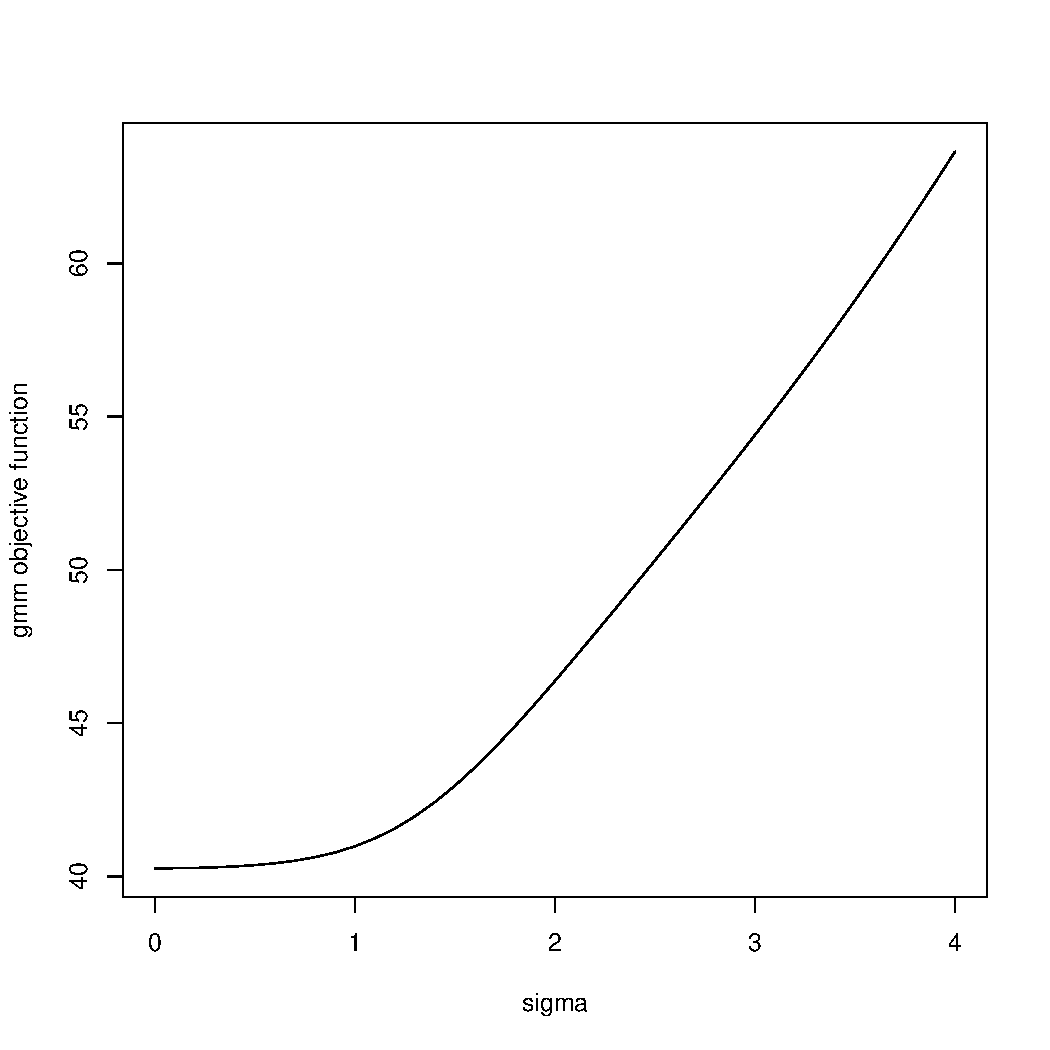
\includegraphics[width=0.8\textwidth]{../Results/Figures/gmm_obj_iv_local.pdf}
    \caption{GMM objective function w.r.t. $\sigma$}
    \label{fig:iv_local_diff}
\end{figure}
The estimation results by regressing $\delta_j$ on $X_j$ and $p_j$ are shown in Table \ref{tab:reg_rand_coef}.
\begin{table}[h!]\fontsize{10pt}{12pt}\selectfont
    \centering
    
\begingroup
\centering
\begin{tabular}{lc}
   \tabularnewline \midrule \midrule
   Dependent Variable:            & y\\  
   Model:                         & (1)\\  
   \midrule
   \emph{Variables}\\
   Constant                       & -1.741\\   
                                  & (1.938)\\   
   p                              & -0.0870$^{**}$\\   
                                  & (0.0428)\\   
   dpm                            & -20.46$^{***}$\\   
                                  & (5.398)\\   
   door3TRUE                      & -0.6440$^{***}$\\   
                                  & (0.2082)\\   
   door4TRUE                      & -0.0094\\   
                                  & (0.1522)\\   
   door5TRUE                      & 0.4822\\   
                                  & (0.3175)\\   
   at                             & -0.2956\\   
                                  & (0.2242)\\   
   ps                             & 0.2206\\   
                                  & (0.1728)\\   
   air                            & 0.5580$^{*}$\\   
                                  & (0.2874)\\   
   drv                            & 0.0961\\   
                                  & (0.1538)\\   
   wt                             & -0.0023$^{***}$\\   
                                  & (0.0006)\\   
   hp2wt                          & -10.12$^{***}$\\   
                                  & (3.726)\\   
   hp                             & 0.0421$^{***}$\\   
                                  & (0.0134)\\   
   euro                           & -1.212$^{***}$\\   
                                  & (0.4153)\\   
   japan                          & 0.0573\\   
                                  & (0.2280)\\   
   wb                             & -0.0207\\   
                                  & (0.0225)\\   
   \midrule
   \emph{Fit statistics}\\
   Observations                   & 501\\  
   Adjusted R$^2$                 & 0.69806\\  
   F-test (1st stage), p          & 4.6944\\  
   F-test (1st stage), p-value, p & $2.99\times 10^{-7}$\\   
   Sargan                         & 72.714\\  
   Sargan, p-value                & $3.71\times 10^{-11}$\\   
   \midrule \midrule
   \multicolumn{2}{l}{\emph{Clustered (modelid) standard-errors in parentheses}}\\
   \multicolumn{2}{l}{\emph{Signif. Codes: ***: 0.01, **: 0.05, *: 0.1}}\\
\end{tabular}
\par\endgroup



    \caption{Random coefficient on size}
    \label{tab:reg_rand_coef}
\end{table}

\section{Question 4+5 : Markups, merger simulation}
\subsection{Price setting equation}
The profit of a multiproduct firm is $$ \Pi_f = \sum_{j\in \mathcal{J}_f} (p_j
    -c_j )s_jM$$ since $s_jM$ represents the sales of the product $j$.

The optimal price is given by taking the first order derivative wrt p.

$$ s_j+\sum_{k\in \mathcal{J}_f} \frac{\partial s_k}{\partial p_j} (p_k-c_k) = 0 \quad \forall j\in \mathcal{J}_f$$

The first term is the direct impact of changing $p_j$. The second term is the
impact on the profits of other products of the firm.

For firm $f$, the pricing equation written in the matrix form gives, $$ S^f +
    \Omega^f(P^f-C^f) = 0$$ where $\Omega^f$ is the matrix of cross-price
elasticities. For example, if firm $f$ has two products, the matrix is $$
    \Omega^f =\begin{bmatrix}
        \frac{\partial s_1}{\partial p_1} & \frac{\partial s_1}{\partial p_2} & 0 \\\ \frac{\partial s_2}{\partial p_1} &\frac{\partial s_2}{\partial p_2} & 0 \\0 & 0 &0\\
    \end{bmatrix}$$

Therefore, aggregate the pricing equation for all firms, we have $$ S + \Omega
    \odot O (P-C) = 0 $$ where $O$ is the ownership matrix.
\subsection{Estimation}
We take $\hat{\alpha}=-0.0785$. We estimate marginal cost (negative), markup
and elasticiy for each year. We simulate a merger between firm17 and firm7, by
modifying the ownership matrix. The mean results are shown in Table
\ref{tab:post_merger_mean}. Table \ref{tab:markup} shows the results.
% latex table generated in R 4.2.1 by xtable 1.8-4 package
% Sat Nov  2 15:53:35 2024
\begin{table}[ht]
\centering
\begin{tabular}{rrrrrrr}
  \hline
 & year & p & mc & mk & elas & p\_new \\ 
  \hline
1 & 1977 & 9.89 & -2.73 & 12.62 & -124.46 & 9.89 \\ 
  2 & 1978 & 10.67 & -1.95 & 12.61 & -134.01 & 10.67 \\ 
  3 & 1979 & 10.50 & -2.06 & 12.56 & -131.42 & 10.50 \\ 
  4 & 1980 & 10.71 & -1.82 & 12.53 & -133.78 & 10.71 \\ 
  5 & 1981 & 12.42 & -0.06 & 12.48 & -154.55 & 12.42 \\ 
   \hline
\end{tabular}
\label{tab:post_merger_mean}
\end{table}
 The anomaly is that we get
negative marginal cost, this is due to the small $\hat{\alpha}$ from the
estimation. Also, the effect of average price seems to be very insignificant.

We calculate consumer surplus pre and post merger in monetary terms, $$CS_i =
    E(\max_j u_{ij})= \frac{\ln(1+\sum_j \exp(\delta_j+\mu_{ij}))}{\alpha_i}$$
Notice that $$s_0=\frac{1}{1+\sum_j \exp\delta_j+\mu_{ij}}$$ Thus
$$CS_i=\frac{-\ln(s_0)}{\alpha_i}$$ In total, $$ CS = M\int
    CS_i(\theta)dF(\theta)$$

The result is shown in Table \ref{tab:post_merger_cs}
% latex table generated in R 4.3.1 by xtable 1.8-4 package
% Sat Nov  2 19:16:50 2024
\begin{table}[ht]
\centering
\begin{tabular}{rrrrrrrr}
  \hline
 & year & nb\_hh & shr\_0 & shr\_0\_new & cs\_pre & cs\_post & diff \\ 
  \hline
1 & 1977 & 74142 & 0.88 & 0.92 & 113392.09 & 74255.59 & -39136.50 \\ 
  2 & 1978 & 76030 & 0.88 & 0.91 & 109959.37 & 84723.89 & -25235.48 \\ 
  3 & 1979 & 77330 & 0.89 & 0.92 & 99446.89 & 72200.37 & -27246.52 \\ 
  4 & 1980 & 80776 & 0.91 & 0.94 & 88677.33 & 59681.78 & -28995.55 \\ 
  5 & 1981 & 82368 & 0.91 & 0.93 & 86013.23 & 64848.35 & -21164.88 \\ 
   \hline
\end{tabular}
\end{table}


% \section{Data and Estimation}
% \subsection{Data}

% The data utilized in this study is from The Annual Statistics of Health
% Establishments (SAE), a comprehensive and mandatory administrative survey that
% serves as the primary source of data on all health establishments in France
% \footnote{\href{https://data.drees.solidarites-sante.gouv.fr/explore/dataset/708_bases-statistiques-sae/information/}{La
%         Statistique annuelle des établissements (SAE)}}. Our analysis primarily focuses
% on healthcare outputs (across eight different measures) and labor inputs (the
% total number of registered and assistant nurses). The panel data spans nine
% years, from 2013 to 2022, excluding 2020 due to disruptions caused by the
% pandemic. The SAE data categorizes establishments into three types based on
% their legal status:

% \begin{enumerate}
%     \item Public hospitals,
%     \item Private for-profit hospitals,
%     \item Private non-profit hospitals.
% \end{enumerate}

% In alignment with the categorization used by \citet{croiset2024hospitals}, this
% study also distinguishes public teaching hospitals as a separate category,
% given their unique role within the French healthcare system.

% \begin{table}[h!]\fontsize{10pt}{12pt}\selectfont
%     \begin{adjustbox}{width=\textwidth,center}
%         \centering
%         \input{../../Tables/Descriptive/hospital_count.tex}
%     \end{adjustbox}
%     \caption{Number of hospitals in each category, 2013-2022}
%     \label{tab:hospital_count}
% \end{table}

% As illustrated in Table \ref{tab:hospital_count}, the distribution of
% hospitals—categorized as normal public, private for-profit, and private
% non-profit—is relatively equal and remains stable over the years. It is
% important to highlight the unique role of teaching hospitals. Unlike other
% types of hospitals, teaching hospitals allocate significant resources to doctor
% training and research activities. This additional commitment to educational and
% research missions generally results in larger institutions. This aspect becomes
% evident when examining the output shares of hospitals in Table
% \ref{tab:nonadjusted}. Despite their limited number, teaching hospitals
% contribute a disproportionately large share of overall healthcare output, a
% disparity that becomes more pronounced when adjusted for the number of
% facilities, as detailed in Table \ref{tab:output}.

% Furthermore, the analysis reveals distinct differences in the mix of service
% provided by each type of hospital. Emergency care is mostly taken care of by
% public hospitals and private hospitals are strong in medical sessions.

% \begin{table}\fontsize{10pt}{12pt}\selectfont
%     \begin{adjustbox}{width=\textwidth,center}
%         \centering
%         \begin{threeparttable}[b]

%             \input{../../Tables/Descriptive/output_share_nonweighted.tex}
%             \caption{Hospital share of output, 2013-2022}
%             \label{tab:nonadjusted}
%         \end{threeparttable}
%     \end{adjustbox}
% \end{table}

% \begin{table}\fontsize{10pt}{12pt}\selectfont
%     \centering
%     \begin{adjustbox}{width=\textwidth,center}
%         \begin{threeparttable}[b]
%             \input{../../Tables/Descriptive/output_share.tex}
%             \caption{Hospital share of output weighted by the number of hospitals, 2013-2022}
%             \label{tab:output}
%             \begin{tablenotes}[para,flushleft]
%                 \footnotesize
%                 \textit{Note:} For example, the value $a_{ij}$ where $i$ is STAC inpatient and $j$ is teaching hospitals, is calculated by $a_{ij}= \frac{\text{Number of STAC inpatient  in teaching hospitals}}{\text{Share of teaching hospitals}\times \text{Total number of STAC inpatient}}$.
%             \end{tablenotes}

%         \end{threeparttable}
%     \end{adjustbox}

% \end{table}

% % proofread until here
% \subsection{Estimation}

% \paragraph{Regression without individual fixed effect}

% The relationship between the number of nurses and output levels in hospitals is
% quantified via a log-log regression specification as follows:

% \begin{equation}
%     \log(x_{it}) = \beta_0 + \beta_1 \log(y_{it}) + \varepsilon_{it}
% \end{equation}

% where $\log(x_{it})$ represents the log of the number of nurses at hospital $i$
% in time $t$, and $\log(y_{it})$ denotes the log of a vector of output levels
% for the same hospital at the same time.

% The regression analysis was conducted separately for each type of hospital, as
% detailed in Table \ref{tab:reg_sep}. The results reveal that teaching hospitals
% have significantly different coefficients compared to other hospital
% categories. This variance is consistent with the unique characteristics of
% teaching hospitals, which were previously noted in their descriptive statistics
% and operational roles.

% Specifically, the deviation in coefficients suggests fundamental differences in
% the input demand functions or, equivalently, in their production functions.
% These differences underscore the distinct operational and functional framework
% within which teaching hospitals operate, further evidenced by their dual focus
% on healthcare delivery and educational responsibilities.

% For this reason, \textbf{teaching hospitals will be excluded from subsequent
%     analyses}. The focus will be on the remaining three categories of hospitals:
% ordinary public hospitals, private for-profit hospitals, and private non-profit
% hospitals.

% \begin{table}[h!]
%     \centering
%     \input{../../Tables/2013-2022/reg_sep_iv.tex}
%     \caption{Separate estimation of input demand function, lagged value as IV, 2013-2022}
%     \label{tab:reg_sep}
% \end{table}

% By excluding teaching hospitals from the analysis, we can more reasonably
% assume that the remaining hospitals share a homogeneous set of coefficients.
% This assumption underpins the pooled regression model, the results of which are
% presented in Table \ref{tab:reg_dummy_iv_ex}. The model incorporates dummy
% variables and uses lagged values as instrumental variables.

% \begin{table}[h!]
%     \centering
%     \input{../../Tables/2013-2022/reg_dummy_iv_ex.tex}
%     \caption{Pooled regression with dummy variables, lagged value as IV, 2013-2022}
%     \label{tab:reg_dummy_iv_ex}
% \end{table}

% At first glance, it appears that private sectors are indeed more efficient in
% labor use. In the next section, I will delve into comparisons between
% individual hospitals and investigate their selection outcomes.

% \paragraph{Regression with individual fixed effect}

% Let $\log(x_{it})$ and $\log(y_{it})$ be defined as previously. Additionally,
% let $\theta_i$ represent the fixed effect for hospital $i$, where $\theta_i$
% can be interpreted as a measure of labor inefficiency. Specifically, a smaller
% $\theta_i$ indicates greater efficiency in labor use by the hospital. These
% fixed effects, $\theta_i$, will be instrumental in ranking and selecting
% hospitals in the subsequent analysis. The model can be specified as follows:

% \begin{equation}
%     \log(x_{it}) = \beta_0 + \beta_1 \log(y_{it}) + \theta_i + \varepsilon_{it}
% \end{equation}

% I considered four types of estimator, within-group, first difference, fist
% difference GMM, system GMM. For expository purposes, the linear specification
% takes the general form of
% \begin{equation*}
%     y_{it} = x_{it} \beta +\theta_i + \epsilon_{it}\quad \text{where} \quad E[\epsilon_{it}|x_{i1},\ldots, x_{it-1},\theta_i]=0.
% \end{equation*}

% The system GMM estimator utilizes two types of moment conditions. The first
% mirrors those used in the first difference GMM estimator:
% \[E[x_{i,t-2}(\Delta y_{it}-\beta\Delta x_{it})]\]
% with lagged $x_{i,t-2}$ serving as an instrument for $\Delta x_{it}$.

% However, if there is high persistency in \( x_{it} \), such that \( x_{it} =
% \alpha x_{i,t-1} + \eta_{it} \) with \( \alpha \) close to 1, this affects the
% strength of the instruments used in the estimation. In this scenario, the
% reduced form relationship between \( \Delta x_{it} \) and \( x_{i,t-2} \) can
% be expressed as:

% \begin{equation*}
%     \Delta x_{it} = (\alpha-1)\alpha x_{i,t-2} + \alpha \eta_{i,t-1} + \eta_{it}
% \end{equation*}

% This relationship posits a challenge in GMM estimation due to the potential
% issue of weak instruments.

% The second moment condition makes another assumption, requiring that the
% correlation between $x_{it}$ and $\theta_i$ is the same as that between
% $x_{i,t-1}$ and $\theta_i$,
% \begin{equation*}
%     \E[\Delta x_{i,t-1}(y_{it}-\beta x_{it})] \quad \text{if}\quad \E\bra{\Delta x_{i,t-1}(\theta_i+\varepsilon_{i,t})}=0
% \end{equation*} where the current level $x_{it}$ is instrumented by lagged first difference $\Delta x_{i,t-1}$.

% Table \ref{tab:reg_wg_fd_gmm} shows that there's a large difference between the
% first difference GMM and system GMM, a sign that the second moment condition
% needs more investigation. Though the estimate from first difference GMM looks
% more hopeful, the Sargan-Hansen test almost rejects the over-identification
% null hypothesis for sure, indicating that some moment conditions are not in
% accordance with each other. Though the issues of weak instruments and rejection
% of over-identification are intriguing problems, I will set them aside for
% future investigation as time allows. I will take as given the estimation
% results from the third column of Table \ref{tab:reg_wg_fd_gmm} and proceed to
% the next section.

% \begin{table}
%     \input{../../Tables/2013-2022/reg_wg_fd_gmm_a.tex}
%     \caption{Estimation of input demand function with individual fixed effect, 2013-2022}
%     \label{tab:reg_wg_fd_gmm}
% \end{table}

% % \begin{table}
% %     \input{../../Tables/2013-2022/reg_wg_fd_iv.tex}
% %     \label{tab:reg_wg_fd_iv}
% % \end{table}

% \section{Compound Decision and Empirical Bayes}

% \subsection{Compound decision framework}
% The idea of compound decision theory was pioneered by
% \citet{robbins1956empirical}. This approach considers the consequences of all
% individual decisions collectively. Consider the scenario where each individual
% unit is associated with an unobserved parameter \( \theta_i \). We are provided
% with a list of estimates \( \hat{\theta}_i \) for each \( \theta_i \).

% \begin{equation*}
%     \boldsymbol{\hat{\theta}}  =  (\hat{\theta}_1,\ldots, \hat{\theta}_n)\quad
%     \text{where} \quad        \hat{\theta}_i | \theta_i \sim P_{\theta_i}
% \end{equation*}

% For the moment, I will remain agnostic about the specific decision to make and
% denote the decision rule by \( \delta \).
% \begin{equation*}
%     \delta(\boldsymbol{\hat{\theta}}) = (\delta_1(\boldsymbol{\hat{\theta}}), \ldots, \delta_n(\boldsymbol{\hat{\theta}}))
% \end{equation*}

% The next step is to define the loss function as the objective function to
% minimize. Since I care about the \textbf{collective performance} of my
% decision, I will define the loss function such that it reflects attention to
% the compound decision. A natural choice would be to aggregate the individual
% losses. Therefore, the compound loss function is defined as:

% \begin{equation*}
%     L_n(\theta, \delta(\boldsymbol{\hat{\theta}})) = \sum_{i=1}^n L(\theta_i, \delta_i(\hat{\theta})).
% \end{equation*}

% Correspondingly, the compound risk is defined as the expectation of the
% compound loss.
% \begin{equation*}
%     R_n(\theta, \delta(\boldsymbol{\hat{\theta}})) = \E_{\theta|\hat{\theta}}[L_n(\theta, \delta(\boldsymbol{\hat{\theta}}))]
% \end{equation*}
% We further restrict our attention to the separable decision rule \( \delta(\boldsymbol{\hat{\theta}}) = \{t(\hat{\theta}_1), \ldots, t(\hat{\theta}_n)\} \). In order to make the connection with the Bayesian view, under which we assume that \( \theta \sim G \), we can rewrite the compound risk as:
% \begin{equation*}
%     R_n(\theta, \delta(\boldsymbol{\hat{\theta}})) = \int \int L(\theta_i, t(\hat{\theta}_i))dP_{\theta_i}(\hat{\theta}_i)dG_n(\theta)
% \end{equation*}
% where $G_n(\theta)$ is the empirical distribution of $\theta$. \footnote{$E_{G_n}(f(x)) = 1/n \sum_i f(x_i)$}

% The Frequentist and Bayesian views differ slightly here in the definition of
% risk. The original compound decision formulation retains the empirical
% distribution \( G_n \) in the compound risk, while the Bayesian risk replaces
% it with the prior distribution \( G \). On a side note, the two views are
% somewhat related to the fixed/random effect terminology, in the sense that the
% fixed effect view treats \( \theta_i \) as fixed unknown parameters, while the
% random effect view treats \( \boldsymbol{\theta} \) as a random draw from a
% distribution \( G \). However, in our context, this distinction has nothing to
% do with whether \( \theta_i \) is correlated with \( x_{it} \).

% The final step involves identifying the decision rule \( \delta^* \) that
% minimizes the risk:
% \begin{equation}
%     \delta^* = \arg \min_{\delta} R_n(\theta, \delta(\boldsymbol{\hat{\theta}}))
% \end{equation}
% subject to any constraints that we might have. Since \( G \) is unknown, the choice between using \( G_n \) or \( G \) for assessing risk is not particularly critical. For the remainder of this section, I will use the Bayesian risk as the minimization objective and apply constraints that are pertinent to the selection problem. Next, I will focus on the non-parametric estimation of the prior distribution \( G \).

% \subsection{Estimate $G$}

% \paragraph{Parametric $G$}

% Most literature has imposed a parametric form of $G$. In the case of a Gaussian
% $G$, recall the hierarchical model
% \begin{align*}
%     \hat{\theta}_i|\theta_i, \sigma_i \sim P_{\theta_i} \\
%     \theta\sim \caln(\mu_\theta,\sigma^2_\theta)
% \end{align*}
% There are two hyperparameters to be estimated $\mu_\theta$ and $\sigma_\theta$.
% % A common estimator would be 
% % \begin{align*}
% %     \hat{\mu}_\theta&=\frac{1}{N} \sum_{i}\hat{\theta}_i\\
% %     \hat{\sigma}_\theta^2&=\frac{1}{N} \sum_{i} \bra{(\hat{\beta}_i-\hat{\mu}_\theta)^2-\sigma_i^2}
% % \end{align*}

% If we compare the performance of the posterior mean estimator \( \theta^* =
% \mathbb{E}[\theta | \hat{\theta}] \) with the original estimate \( \hat{\theta}
% \), \citet{james1992estimation} has shown that there is always an improvement
% in average performance if we assume \( G \) is Gaussian and replace it with an
% estimate \( \hat{G} \). If we relax the normality assumption on \( G \) and
% adopt a nonparametric maximum likelihood estimation (NPMLE) as established by
% \citet{kiefer1956consistency}, there could be further improvements. For
% example, \citet{jiang2009general} has proven that a plugged-in \( \theta^* \)
% with a NPMLE \( \hat{G} \) is asymptotically optimal among all separable
% estimators. A comparison between the parametric and non-parametric \( \hat{G}
% \) is demonstrated in \citet{gilraine2020new} on their teacher value-added
% application.

% \paragraph{Nonparametric $G$}

% The initial NPMLE (Nonparametric Maximum Likelihood Estimator) as defined by
% \citet{kiefer1956consistency} takes the following form:
% \begin{equation*}
%     \hat{G} = \argmin_{G \in \mathcal{G}} \left\{-\sum_{i=1}^{n}\log g(y_i) \mid g(y_i) = \int \p(y_i |\theta) dG(\theta) \right\}
% \end{equation*}
% where \( \p(y_i |\theta) \) represents the probability density function of \( y_i \) conditional on the true parameter \( \theta \), and \( g(y_i) \) is the marginal pdf of \( y_i \).

% This optimization problem is convex, featuring a strictly convex objective and
% a convex constraint set. However, it involves an infinite-dimensional parameter
% space. To tackle the primal problem, it is necessary to discretize it.

% The algorithm proposed by \citet{koenker2014convex} utilizes the interior point
% method, a technique frequently employed in convex optimization implemented by
% \verb+MOSEK+ \citep{andersen2010mosek}. This approach significantly enhances
% computational efficiency compared to the fixed point EM iteration method
% previously suggested by \citet{jiang2009general}. This advancement in
% computational strategies has made the implementation of the Nonparametric
% Maximum Likelihood Estimator (NPMLE) more practical and faster for applied
% statistical analysis, offering a robust alternative for dealing with complex
% data models where traditional methods may falter.

% % proofread til here

% \section{The Selection Problem}
% \subsection{Definition}
% The definition of the selection problem is taken from the work of
% \citet{gu2023invidious}. Instead of focusing on the right tail of the
% distribution, the top performers in my context correspond to the left tail. The
% task at hand is to select the bottom 20\% of the \( \theta_i \) and compare the
% share of public and private sectors in the meritorious group. This offers
% another perspective on the public and private sectors, different from that of
% \citet{croiset2024hospitals}.

% In addition to the constraint on the size of the selected group (20\%), I have
% further imposed a constraint on the number of false positive mistakes made in
% the selection process. This leads to the implementation of a false discovery
% constraint at level \( \gamma \).
% \begin{equation*}
%     \frac{\E_G\bra{h_i=0,\delta_i=1}}{\E_G\bra{\delta_i}} \le \gamma
% \end{equation*} where $h_i=1\set{\theta_i<\theta_\alpha}$ is the indicator function of whether the unit $i$ is truly below the threshold $\theta_\alpha$. And $\delta_i=1$ when unit $i$ is selected.

% All in all, we can formally define the loss function of selection problem as
% \begin{equation*}
%     L(\delta,\theta)=\sum_i h_i(1-\delta_i) +\tau_1\pa{\sum_i (1-h_i)\delta_i -\gamma \delta_i} + \tau_2 \pa{\sum_i \delta_i -\alpha n}
% \end{equation*}
% and the optimal decision rule is given by
% \begin{equation} \label{eq:decisionrule}
%     \begin{split}
%         \delta^* & =\argmin_\delta \E_G\E_{\theta|\hat{\theta}}\bra{L(\delta,\theta)}                                                                                                              \\
%         & = \E_G \ \sum_i \E_{\theta|\hat{\theta}}(h_i)(1-\delta_i) +\tau_1\pa{\sum_i (1-\E_{\theta|\hat{\theta}}(h_i))\delta_i -\gamma \delta_i} + \tau_2 \pa{\sum_i \delta_i -\alpha n} \\
%         & =\E_G{\sum_i v_\alpha(\hat{\theta})(1-\delta_i) +\tau_1\pa{\sum_i (1-v_\alpha(\hat{\theta}))\delta_i -\gamma \delta_i} + \tau_2 \pa{\sum_i \delta_i -\alpha n}}
%     \end{split}
% \end{equation}

% Here, the term \(\E_{\theta|\hat{\theta}}(h_i)\) is called \textbf{posterior
%     tail probability}. It is the probability of \(i\) being truly in the bottom
% \(\alpha\%\) given the estimated \(\hat{\theta}\). This is a posterior
% statistic different from the posterior mean
% \(\E_{\theta|\hat{\theta}}(\theta_i)\) because the variable inside the
% expectation \(h_i = 1\{\theta_i < G^{-1}(\alpha)\}\) is specific to the
% capacity constraint at the \(\alpha\) level. From the previous section, we have
% obtained an estimate of the prior distribution \(G\) so that we can derive the
% posterior tail probability \(v_\alpha(\hat{\theta}_i)\).

% \begin{equation*}
%     v_\alpha=P( \theta_i < \theta_{\alpha} |\hat{\theta})
% \end{equation*}

% If we know that \(\hat{\theta}|\theta \sim P_\theta\) with density function
% \(p_\theta\), the posterior tail probability can be further expressed as:
% \begin{equation*}
%     v_\alpha(y_i) = \frac{\int_{-\infty}^{\theta_{\alpha}} p_{\theta_i}(y_i) dG(\theta_i)}
%     {\int_{-\infty}^{\infty} p_{\theta_i}(y_i) dG(\theta_i)}
% \end{equation*}

% From now on, the notation \(\hat{\theta}_i\) is replaced by \(y_i\). For
% example, if \(y_i|\theta_i \sim \mathcal{N}(\theta_i, \sigma_i^2)\), as is
% often the case in applications, \(v_\alpha\) takes the explicit form:
% \begin{equation*}
%     = \frac{\int_{-\infty}^{\theta_{\alpha}} \varphi(y_i | \theta_i, \sigma_i^2) dG(\theta_i)}
%     {\int_{-\infty}^{\infty} \varphi(y_i | \theta_i, \sigma_i^2) dG(\theta_i)}
% \end{equation*}
% where \(\varphi\) is the density function of \(y_i\) with conditional mean \(\theta_i\) and variance \(\sigma_i^2\).

% Here, we have assumed that \(\sigma_i\) is known, meaning that \(P_\theta\)
% only depends on \(\theta_i\). However, sometimes \(\sigma_i\) is unknown,
% meaning that \(P_\theta\) depends on additional parameters. These two cases
% must be distinguished when defining the posterior tail probability and
% constraints.

% The two constraints can be preliminarily written out as follows:
% \begin{itemize}
%     \item Capacity constraint: \[ \p(v_\alpha>\lambda_1^*) \le \alpha \Rightarrow \lambda_1^* = H^{-1}(1-\alpha). \] Empirically, $\lambda_1^*$ is found by the inverse function of the empirical
%           cumulative distribution $H$ of $v_\alpha$ at $1-\alpha$.
%     \item False Discovery constraint: \[ \p(\theta<\theta_\alpha|v_\alpha>\lambda_2^*) \le \gamma \Rightarrow  \frac{\sum_i \E[(1-v_{\alpha,i})\delta_i]}{\sum_i E[ \delta_i]}\le \gamma.\] First, We approximate $\p(\theta<\theta_\alpha|v_\alpha>\lambda_2^*)$ by
%           $\frac{\sum_i E[ (1-h_i)\delta_i]}{\sum_i E[ \delta_i]}$. Then it needs to be
%           shown that $\E[ (1-h_i)\delta_i]$ is equivalent to
%           $\E[(1-v_{\alpha,i})\delta_i]$. This is straightforward by the law of iterated
%           expectation. Let $D_i = (Y_i,\sigma_i^2)$ when $\sigma_i^2$ is known and $D_i =
%               (Y_i,S_i)$ when $\sigma_i^2$ is unknown.
%           \[ \E[(1-h_i)\delta_i] = \E[\E[(1-h_i)\delta_i|D_i]] = \E[\delta_i(1-\E[h_i|D_i])] = \E[\delta_i(1-v_{\alpha,i})] \]
% \end{itemize}
% These formulations allow us to control the size of the selected group while also maintaining the expected rate of false discoveries within an acceptable level \(\gamma\).

% Now, we will critically distinguish between the two scenarios where
% \(\sigma_i\) is known and unknown. The posterior tail probability and
% constraints are defined accordingly.

% \paragraph{Known variance, $G(\theta)$}
% The true inefficiency value of hospital $i$ is $\theta_i$, We only observe a
% sequence of $Y_{i}$ where
% \begin{equation*}
%     Y_{i} = \theta_i + \varepsilon_{it} \quad \varepsilon_{it} \sim \caln(0,\sigma_i^2) \quad (\theta_i) \sim G
% \end{equation*}
% The tail probability $v_\alpha$ is a function of $y_i$ only
% \begin{equation*}
%     v_\alpha(y_i) =\p(\theta_i<\theta_\alpha|y_i) =\frac{\int_{-\infty}^{\theta_\alpha} \varphi(y_i|\theta_i,\sigma_i^2)dG(\theta_i)}{\int \varphi(y_i|\theta_i,\sigma_i^2)dG(\theta_i)}
% \end{equation*}
% The cutoff $\lambda^*$ is determined such that the constraints are satisfied
% \begin{align*}
%     \p(v_\alpha>\lambda^*) \le \alpha \\
%     \p(\theta<\theta_\alpha|v_\alpha>\lambda^*) \le \gamma
% \end{align*}

% \paragraph{Unknown variance, $G(\theta,\sigma)$}
% We only observe a sequence of $Y_{it}$ where
% \begin{equation*}
%     Y_{it} = \theta_i + \varepsilon_{it} \quad \varepsilon_{it} \sim \caln(0,\sigma_i^2) \quad (\theta_i,\sigma_i^2) \sim G
% \end{equation*}
% Neither $\theta_i$ nor $\sigma_i^2$ is known. But there exists two sufficient statistics for $(\theta_i,\sigma_i)$ such that
% \begin{align*}
%     Y_i=\frac{1}{T_i}\sum_{t=1}^{T_i}Y_{it}           & \quad \text{where}\quad Y_i|\theta_i,\sigma_i^2 \sim \caln(\theta_i,\sigma_i^2/T_i)              \\
%     S_i=\frac{1}{T_i-1}\sum_{t=1}^{T_i}(Y_{it}-Y_i)^2 & \quad \text{where} \quad S_i|\sigma_i^2 \sim \Gamma(\frac{(T_i-1)}{2},\frac{2\sigma_i^2}{T_i-1})
% \end{align*}

% Now the posterior tail probability $v_\alpha$ is a function of both $y_i$ and
% $s_i$
% \begin{align*}
%     v_\alpha(y_i,s_i) & =\p(\theta_i<\theta_\alpha|y_i,s_i)                                                                                                                                                                                                                                                                \\
%                       & =\frac{\int\int_{-\infty}^{\theta_\alpha} \Gamma(s_i|\frac{(T_i-1)}{2},\frac{2\sigma_i^2}{T_i-1})\varphi(y_i|\theta_i,\frac{\sigma_i^2}{T_i})dG(\theta,\sigma^2)}{\int\int \Gamma(s_i|\frac{(T_i-1)}{2},\frac{2\sigma_i^2}{T_i-1})\varphi(y_i|\theta_i,\frac{\sigma_i^2}{T_i})dG(\theta,\sigma^2)} \\
% \end{align*}

% The cutoff $\lambda^*$ is found in the same way as before.

% \subsection{Results}

% Having defined the selection problem, I will now present the results by
% incorporating empirical estimation of the prior distribution \( G \).

% To ensure the variability of the data, I have selected hospitals with than 6
% years of observations. In the end, the sample contains 1580 hospitals, out of
% which 604 are public hospitals and 976 are private ones. The $Y_{it}$ in the
% last section is calculated as $ \log(x_{it,\text{nurses}}) -
%     \log(y_{it,\text{output}})\hat{\beta}$. Since the panel is too short to invoke
% central limit theorem, I am obliged to impose normality assumption on the error
% term $\varepsilon \sim \caln(0,\sigma_i^2)$ in order to apply the results
% above. Thus, $Y_{it}$ follows a normal distribution
% $\caln(\theta_i,\sigma_i^2)$ as the number of hospitals $N$ tends to infinity.

% Instead of assuming that $\sigma_i^2$ (or the distribution of it) is known, in
% our setting it seems more reasonable to employ the estimates of it $S_i$ in
% defining $v_\alpha$. However, in empirical studies such as baseball batting
% averages \citep{gu2017empirical}, teacher added value \citep{gilraine2020new}
% and kidney dialysis center rating \citep{gu2023invidious}, an estimate of the
% variance is taken to be the true value. A comparison of selection results under
% the two different assumptions will be presented in this section.

% \paragraph{Unknown variance, and TP rules}

% Since we only observe the sample mean $Y_i$ and sample variance $S_i$, the
% prior $G$ is a two-dimensional distribution on $(\theta,\sigma^2)$. Without
% assuming independence between the two parameters, we can utilize a
% two-dimensional gridding strategy in defining the convex objective function:

% \begin{equation*}
%     \hat{G}=\argmin_{G\in \mathcal{G}} \set{-\sum_{i=1}^{n}\log g(y_i,s_i)|g(y_i,s_i)=\int \int  \p(y_i,s_i |\theta,\sigma^2)dG(\theta,\sigma^2) }
% \end{equation*}

% This can be solved using the interior point method, similar to the
% one-dimensional case. The solution is an atomic distribution with fewer than
% $n$ atoms. It is worth mentioning that the NPMLE method is self-regularizing
% because the mass points are determined by the solution without the need for any
% tuning parameter. Further smoothing is justified by the fact that we have
% ignored the variability of $G$. The bandwidth of the biweight kernel for
% smoothing was chosen based on the mean absolute deviation from the median of
% the discrete $\hat{G}$.

% The left-hand side of Figure \ref{fig:GLVmix} shows the estimated
% $\hat{G}(\theta, \sigma^2)$ before smoothing, while the right-hand side
% displays the smoothed version.

% \begin{figure}[h!]
%     \centering
%     \begin{minipage}{0.5\textwidth}
%         \centering
%         \includegraphics[width=\textwidth]{../../Figures/2013-2022/GMM_fd/GLVmix.pdf}
%     \end{minipage}\hfill
%     \begin{minipage}{0.5\textwidth}
%         \centering
%         \includegraphics[width=\textwidth]{../../Figures/2013-2022/GMM_fd/GLVmix_s.pdf}
%     \end{minipage}
%     \label{fig:GLVmix}
% \end{figure}

% With an estimated prior, the tail probability function as well as the
% constraints are well-defined. However, given the discrete nature of selection,
% it resembles knapsack discrete optimization problem similar. I follow the
% approach described in \cite{basu2018weighted} and thus consider only
% sequentially selecting the units until one constraint is violated.

% In Figure \ref{fig:tp_0.2_0.2_2d}, I present the results of selecting the top
% 20\% of hospitals with or without the FDR constraint set at 20\%. The selection
% rule is the posterior tail probability, which is explained in the sections
% above, that is, the solution to the problem defined in \ref{eq:decisionrule}.
% The prior $G$ is taken to be the smoothed Kiefer-Wolfowitz estimate.

% The left-hand side corresponds to the selection outcome without imposing the
% FDR constraints, while the right-hand side controls the expected FDR at 20\%.
% In the first case, there are around 10 times more private hospitals in the top
% 20\%, while the total number of hospitals is less than twice that of the
% public.

% The FDR seems to have impacted only the private hospitals, leaving 18 out of
% the selection set. A more stringent FDR constraint would lead to a smaller set,
% as shown in \ref{fig:tp_0.2_0.1_2d}.

% \begin{figure}[h!]
%     \centering
%     \includegraphics[width=0.8\textwidth]{../../Figures/2013-2022/GMM_fd/GLVmix/Left_0.2_0.2_TPKWs.pdf}
%     \caption{Tail probability rule, capacity 20\%, FDR 20\%, unknown variance}
%     \label{fig:tp_0.2_0.2_2d}
% \end{figure}

% \begin{figure}[h!]
%     \centering
%     \includegraphics[width=0.8\textwidth]{../../Figures/2013-2022/GMM_fd/GLVmix/Left_0.2_0.1_TPKWs.pdf}
%     \caption{Tail probability rule, capacity 20\%, FDR 10\%, unknown variance}
%     \label{fig:tp_0.2_0.1_2d}
% \end{figure}

% For an overview of other selection rules using different ranking statistics,
% such as the posterior mean, MLE face value, and James-Stein linear shrinkage,
% see Appendix \ref{section:unknown}.

% \paragraph{Known variance, and TP rules}

% In \citet{gu2023invidious}, the authors apply the newly proposed selection
% method to the selection of kidney dialysis centers, a topic previously studied
% by \citet{lin2006loss, lin2009ranking}. However, their focus is on the quality
% of service, specifically on the mortality rate. Furthermore, they assume that
% the predictions of expected mortality are sufficiently accurate such that the
% variance is known, independent of $\theta \sim G$.

% Figure \ref{fig:GLmix} shows the estimated $\hat{G}(\theta)$ before and after
% smoothing.

% \begin{figure}[h!]
%     \centering
%     \begin{minipage}{0.5\textwidth}
%         \centering
%         \includegraphics[width=\textwidth]{../../Figures/2013-2022/GMM_fd/GLmix.pdf}
%     \end{minipage}\hfill
%     \begin{minipage}{0.5\textwidth}
%         \centering
%         \includegraphics[width=\textwidth]{../../Figures/2013-2022/GMM_fd/GLmix_s.pdf}
%     \end{minipage}
% \end{figure}

% Though not desirable in the present setting, it would be interesting to see
% what the results would be if I take the $S_i$ as the $\sigma_i^2$. For the
% moment, whether this assumption would lead to a more stringent selection
% outcome is unclear. Figure \ref{fig:tp_0.2_0.2_1d} presents the outcome under
% the posterior tail probability rule with a smoothed estimated prior. It seems
% that with only the capacity constraint, the outcome does not differ much.
% However, when an FDR constraint is combined, the known variance assumption
% becomes too lenient to incorporate the newly imposed constraint. At the level
% $\alpha=0.2$ and $\gamma=0.2$, the FDR constraint is not binding. However, a
% more stringent FDR constraint at $\gamma=10\%$ does bind, as shown in Figure
% \ref{fig:tp_0.2_0.1_1d}.

% \begin{figure}[h!]
%     \centering
%     \includegraphics[width=0.8\textwidth]{../../Figures/2013-2022/GMM_fd/GLmix/Left_0.2_0.2_TPKWs.pdf}
%     \caption{Tail probability rule, capacity 20\%, FDR 20\%, known variance}
%     \label{fig:tp_0.2_0.2_1d}
% \end{figure}

% \begin{figure}[h!]
%     \centering
%     \includegraphics[width=0.8\textwidth]{../../Figures/2013-2022/GMM_fd/GLmix/Left_0.2_0.1_TPKWs.pdf}
%     \caption{Tail probability rule, capacity 20\%, FDR 10\%, known variance}
%     \label{fig:tp_0.2_0.1_1d}
% \end{figure}

% Appendix \ref{section:known} presents the results of other selection rules. In
% this case, a contour line can be drawn to highlight the differences between
% ranking statistics.

% \section{Conclusion}
% Exploiting the rich dataset covering all hospitals in France, I have attempted
% to estimate the fixed effect of individual hospitals, which has the
% interpretation of an \textit{inefficiency index}. Based on an initial estimate,
% my goal is to select the top-performing hospitals and classify them by legal
% status, thereby having a more granular view of the efficiency comparison
% between public and private hospitals. I deliberately omit the teaching
% hospitals (approximately 200) from the dataset because they inherently differ
% in terms of objectives. To tackle the endogeneity problem, I used the first
% difference GMM method, though subject to overidentification issue. The
% selection problem of interest falls naturally under the compound decision
% framework. The Empirical Bayes ideology, along with developments in
% non-parametric maximum likelihood estimation, has made the implementation more
% efficient. In addition to the artificial capacity constraint where only the top
% $\alpha\%$ of units are of interest, it is an interesting and useful practice
% to incorporate another constraint called the False Discovery Rate (FDR)
% constraint such that the expected number of false positives is controlled at a
% certain level. From the application to French hospitals, it is clear that the
% FDR constraint shrinks the selection set by some amount. It is also intuitive
% that the larger the capacity (the larger the $\alpha$), the less binding the
% FDR constraint is. The idea is that when the decision-maker can select more
% units, the probability of making mistakes decreases. Another observation comes
% from the assumption we make in the NPMLE of $G$. In \citet{gu2023invidious},
% the authors have pointed out that while the known variance assumption in
% $Y_i|\theta_i,\sigma_i$ may be plausible in some applications, it is more
% common to be faced with only an estimate of the variance. The two assumptions
% give rise to a different level of \textit{stringency} in response to the
% constraints, especially when the decision-maker wants to control for the
% expected false discovery rate. Assuming an unknown variance treats the
% observation as noisier, thus increasing the probability of making mistakes. The
% same level of FDR constraint of 20\% only binds in the unknown variance
% scenario. With respect to the private-public comparison, among the top 20\%
% performers, there are around ten times more private than public hospitals,
% while the ratio of total number is 5 to 3. A preliminary conclusion is that in
% terms of labor employment efficiency, there are more efficient private
% hospitals among the top performers. It may be of interest to healthcare
% authorities to perform such selections and take corresponding actions with
% respect to the selection outcome. From my point of view, a related report based
% on the ranking and selection results will create an incentive for healthcare
% providers to ensure the completeness of data input. However, one cautionary
% note is the interpretation of the fixed effect estimate. Since the fixed effect
% captures all time-invariant components of the unit, whether it is only the
% unobserved heterogeneity of individual hospitals or an actual measure of
% inefficiency is questionable. This issue is discussed in
% \citet{greene2005fixed}. Lastly, despite the fact that it is human nature to
% construct rankings and make selections, every step of the procedure requires
% attention to specification, identification, and justifiable assumptions.
% Incorporating constraints such as FDR in defining the problem may be helpful,
% but the decision is still subject to great uncertainty and should be made with
% caution and justification.

% \pagebreak
% \newpage
% \bibliography{ref.bib}

% \appendix
% \section{Appendix}
% \subsection{Data and Code}

% \paragraph{Data} The panel is first filtered by the following criteria
% \begin{enumerate}
%     \item the number of nurses is positive,
%     \item at least one of STAC inpatient, STAC outpatient, Sessions is positive,
%     \item the number of observations is larger than 6.
% \end{enumerate}
% Second, I add one to every variable to avoid null value when taking log. Third, I only consider units where the estimated variance of the fixed effect is larger than 0.001.

% \paragraph{Code} All implementation details can be found in
% \href{https://github.com/zfuak/RankHospital}{this repository}.

% \subsection{Assumption on $\hat{\theta}_i|\theta_i,\sigma_i$}
% If our specification and assumptions on exogeneity are correct, the consistency
% of $\hat{\beta}$ is guaranteed by $N$'s asymptotic. However, our estimate of
% the fixed effect is
% \begin{align*}
%     \hat{\theta}_i & =\frac{1}{T}\sum(\theta_i+\varepsilon_{it}+x_{it}(\beta-\hat{\beta}))              \\
%                    & \overset{N\to \infty}{\longrightarrow} \theta_i+\frac{1}{T}\sum_t \varepsilon_{it} \\
% \end{align*}
% When $T$ is relatively small (or even fixed), I am not in a good position to use central limit theorem to claim that $\hat{\theta}_i \overset{d}{\to} \caln(\theta_i,\frac{\sigma_i^2}{T})$. A bold assumption that $\varepsilon_{it} \sim \caln(0,\sigma_i^2)$ will save me from the $T$ issue, which I will impose for the rest of the section (and abstract from whether that  for each $i$ is a testable/reasonable/feasible assumption).

% \subsection{NPMLE $G$}
% \citet{koenker2014convex} defined the primal problem as
% \begin{equation*}
%     \min_{f=dG}\set{-\sum_i \log g(y_i)\bigg |g(y_i) = T(f),\ K(f)=1,\ \forall i }
% \end{equation*}
% where $ T(f)=\int p(y_i |\theta)fd\theta $ and  $K(f)= \int f d\theta$.\\
% By discretizing the support,
% \begin{equation*}
%     \min_{f=dG}\left\{-\sum_i \log g(y_i)\bigg |g=Af,\ {1^T}f=1\right\}
% \end{equation*}
% where $A_{ij}= p(y_i|\theta_j) $ and $ f = (f(\theta_1),f(\theta_2),\ldots,f(\theta_m))$.\\
% It is straightforward to derive the dual problem
% \begin{equation*}
%     \max_{\lambda,\mu} \left\{ \sum_i \log \lambda_1(i) \bigg| A^T\lambda_1 < \lambda_2 1,\ (\lambda_1>0) \right\}
% \end{equation*}

% \subsection{Comparison of selection rules}

% \newpage
% \subsubsection{Unknown variance}
% \label{section:unknown}

% \begin{figure}[h!]
%     \centering
%     \includegraphics[width=0.8\textwidth]{../../Figures/2013-2022/GMM_fd/GLVmix/Left_0.2_0.2_PMKWs.pdf}
%     \caption{Posterior mean, capacity 20\%, FDR 20\%, unknown variance}
% \end{figure}

% \begin{figure}[h!]
%     \centering
%     \includegraphics[width=0.8\textwidth]{../../Figures/2013-2022/GMM_fd/GLVmix/Left_0.2_0.2_JS.pdf}
%     \caption{James-Stein Linear Shrinkage, capacity 20\%, FDR 20\%, unknown variance}
% \end{figure}

% \begin{figure}[h!]
%     \centering
%     \includegraphics[width=0.8\textwidth]{../../Figures/2013-2022/GMM_fd/GLVmix/Left_0.2_0.2_MLE.pdf}
%     \caption{MLE, capacity 20\%, FDR 20\%, known variance}
% \end{figure}

% \newpage
% \subsubsection{Known variance}
% \label{section:known}
% \begin{figure}[h!]
%     \centering
%     \includegraphics[width=0.8\textwidth]{../../Figures/2013-2022/GMM_fd/GLmix/Contour_Left_0.2_0.1_TPKWs_PMKWs.pdf}
%     \caption{TP VS PM,  capacity 20\%, FDR 10\%, known variance}
% \end{figure}

% \begin{figure}[h!]
%     \centering
%     \includegraphics[width=0.8\textwidth]{../../Figures/2013-2022/GMM_fd/GLmix/Contour_Left_0.2_0.1_TPKWs_JS.pdf}
%     \caption{TP VS JS, capacity 20\%, FDR 10\%, known variance}
% \end{figure}

% \begin{figure}[h!]
%     \centering
%     \includegraphics[width=0.8\textwidth]{../../Figures/2013-2022/GMM_fd/GLmix/Contour_Left_0.2_0.1_TPKWs_MLE.pdf}
%     \caption{TP VS MLE, capacity 20\%, FDR 10\%, unknown variance}
% \end{figure}

\end{document}